\documentclass[12pt,a4paper]{article}
\usepackage{amsmath,amsthm,amssymb}
\usepackage{array}
\usepackage{latexsym,alltt,varioref,keyval,nameref,verbatim}
\usepackage{color}
\usepackage{amsmath,amsthm,amssymb}
\usepackage{graphics,graphicx}
\usepackage[colorlinks,filecolor=blue,pagebackref,dvips=true]{hyperref}

%\pagestyle{myheadings}
\markright{\protect\pageref{lastpage} pages}

\def \a{\alpha}
\def \d{\partial}
\def \p{\varphi}
\def\E{{\mathbb E}}
\def\D{{\mathbb D}}
\def\P{{\mathbb P}}
\def\Q{{\mathbb Q}}
\def\R{{\mathbb R}}
\def\V{{\mathbb{V}ar}}
\def \L{\mathbb{L}}
\def \cG{\mathcal{G}}
\def \cF{\mathcal{F}}
\def \cS{\mathcal{S}}
\def \cD{\mathcal{D}}
\def \cP{\mathcal{P}}
\def \cL{\mathcal{L}}
\def \cN{\mathcal{N}}

\addtolength{\hoffset}{-1cm}
\addtolength{\textwidth}{2cm}

\begin{document}
\author{Ismail Laachir}
\title{Calibration of the Hull-White Two-Factor Model}
\date{\today}
\maketitle

%\thispagestyle{myheadings}

\tableofcontents

\vspace{10mm}
  
This document describes the Hull White Two Factor model for interest rates and a C implementation in PREMIA of the calibration of this model using the market prices of caps and swaptions.\\

\textit{NB : To know how to run the program, read the file README.}


\section{Model Presentation}

Hull/White model is a short-rate model, it has two version, one-factor and two-factor. One of the main characteristics of this model is its ability to match the initial yield curve by using a shift function and the fact that the two-factor version of the model, unlike the one-factor version, introduces non-trivial correlation between forward rates, which is more realistic in market point of view. In fact, as noticed in \cite{BM}, in HW one-factor model, the correlation between continuously-compound spot rates for two different dates is equal to 1, which mean that a shock to interest rate curve is transmitted equally trough maturities while the two-factor model allows to have a non-perfect correlation, which is closer to market behavior. Having this property, commonly called ``achieving decorrelation'', in a given model is interesting when modeling complex product where correlation plays an important role.\\

Hull/White two-factor model is defined by an SDE which describes the
evolution of the spot rate $r(t)$:
\begin{equation*}
\begin{array}{l}
\left\{
\begin{array}{l}
dr(t)  = \left[ \theta(t)+ u(t) - a \,r(t)\,\right] dt + \sigma_1\,dW_1(t)\\
\\
du(t)  = -b \,u(t)\,dt + \sigma_2\,dW_2(t), \quad u(0)=0\\
\end{array}
\right.
\end{array}
\end{equation*}

The two processes $W_1$ and $W_2$ are brownian motions with instantaneous correlation $\rho$, and $\theta$ is a deterministic function totally given by the market value of the zero coupon bonds.\\

Let us denote by $P_M(0,T)$ the market zero coupon bond value maturing at time
$T$ and $f_M(t)=-\frac{\d log(P_M(0,t))}{\d t}$ the market present
instantaneous forward rate, then with an appropriate choice for the function $\theta$ (see Hull/White 1994 for details), the model exactly fits the market bonds curve and we have several analytical formulas :\\

\noindent Zero coupon bond at time t knowing that $r(t) = r_t$ and $u(t) = u_t$ :

$$P(t,T)  =  A(t,T)e^{-B(t,T)\,r_t-C(t,T)\,u_t}.$$

\noindent Explicit formulations for $A$, $B$ and $C$ can be found in \cite{HW2d}.\\

\noindent The price at time t for a European Call on a ZC bond : 
$$C_t = \E_t \left[ e^{-\int_t^T r(s)ds}(P(T,S)-K)_+ \right] =
P(t,S)\cN(h) -KP(t,T)\cN(h-\sigma_p).$$
Where $\cN$ is the cumulative function of the normal law,
$$h=\frac{1}{\sigma_p}log\left(\frac{P(t,S)}{P(t,T)K}\right)+\frac{\sigma_p}{2}$$ and
$\sigma_p$ is given in \cite{HW2d}.\\

This closed formula for european option on bond leads to closed formula for cap and floor, using the relation bond option and cap/floor. The price of an european swaption is more complicated and takes more time than cap pricing.\\

We finaly notice that the Hull/White 2-factor model is equivalent to the G2++ model by Brigo and Mercurio \cite{BM}. In fact, the parameters of one model can be recovered from the parameters of the other one\footnote{You can use the function void HW2dparams$\_$to$\_$G2dparams(double a, double b, double *sigma, double *eta, double *rho) to transfrom HW2d parameters into G2++ parameters.}. See \cite{BM}, page 161, for formulas.

\section{Model Calibration}

The goal of calibration is to estimate the five parameters of the model $(a, \sigma_1, b, \sigma_2, \rho)$ fitting a given observed market data (cap or swaption implied volatility surface). For purpose of comparison, we consider two examples of calibration to real market volatility data, as in the book of Brigo/Mercurio \cite{BM}\footnote{The comparison is a bit difficult because the initial term structure of zero coupon bond used in \cite{BM} is given in a graphic, so we had to recover the numerical values approximatively from the curve.}. In their book, they considered the so called G2++ model, but it is equivalent to the Hull White 2-factor model, using a relation between the five parameters of the two models (see \cite{BM}, page 161).

\subsection{First example : calibration to cap volatility}

In this example we use the at-the-money Euro cap-volatility that we recall in table \ref{''cap''}. The calibration is performed by minimizing the sum of the squares of the percentage differences between model and market cap prices. For this purpose, we used an optimization algorithm, that we already implemented, proposed by \cite{BFGS} that combines interior point methods and quasi-Newton techniques.\\

The table \ref{''cap''} and graph \ref{fig:cap_vol} reports the results of the calibration to cap volatility.

\begin{table}[''h'']
   \centering
    \begin{tabular}{|c|c|c|c|c|}
    \hline
      \texttt{Maturity} & \texttt{Market Volatility} & \texttt{BM Volatility}& \texttt{Our Volatility}\\
    \hline
1.0   & 0.1520 & 0.1520 & 0.1520 \\ 
2.0   & 0.1620 & 0.1622 & 0.1622 \\ 
3.0   & 0.1640 & 0.1631 & 0.1633 \\ 
4.0   & 0.1630 & 0.1631 & 0.1630 \\ 
5.0   & 0.1605 & 0.1614 & 0.1613 \\ 
7.0   & 0.1555 & 0.1554 & 0.1552 \\ 
10.0  & 0.1475 & 0.1472 & 0.1474 \\ 
15.0  & 0.1350 & 0.1349 & 0.1350 \\ 
20.0  & 0.1260 & 0.1261 & 0.1261 \\ 
    \hline
\end{tabular}
\caption{\label{''cap''} Calibration results for caps. }
\end{table}

These results are obtained with the following Hull/White parameters: 
$$a = 0.521159,\; \sigma_1 = 0.005943,\; b = 0.075631,\;  \sigma_2 = 0.005156,\; \rho = 0.987593 $$
, which are equivalent to the following G2++ parameters, using Brigo/Mercurio notations :
$$a = 0.521159,\; \sigma = 0.005779,\; b = 0.075631,\;  \eta = 0.011573,\; \rho = -0.986876 $$

\begin{figure}[h!]
 \centering
 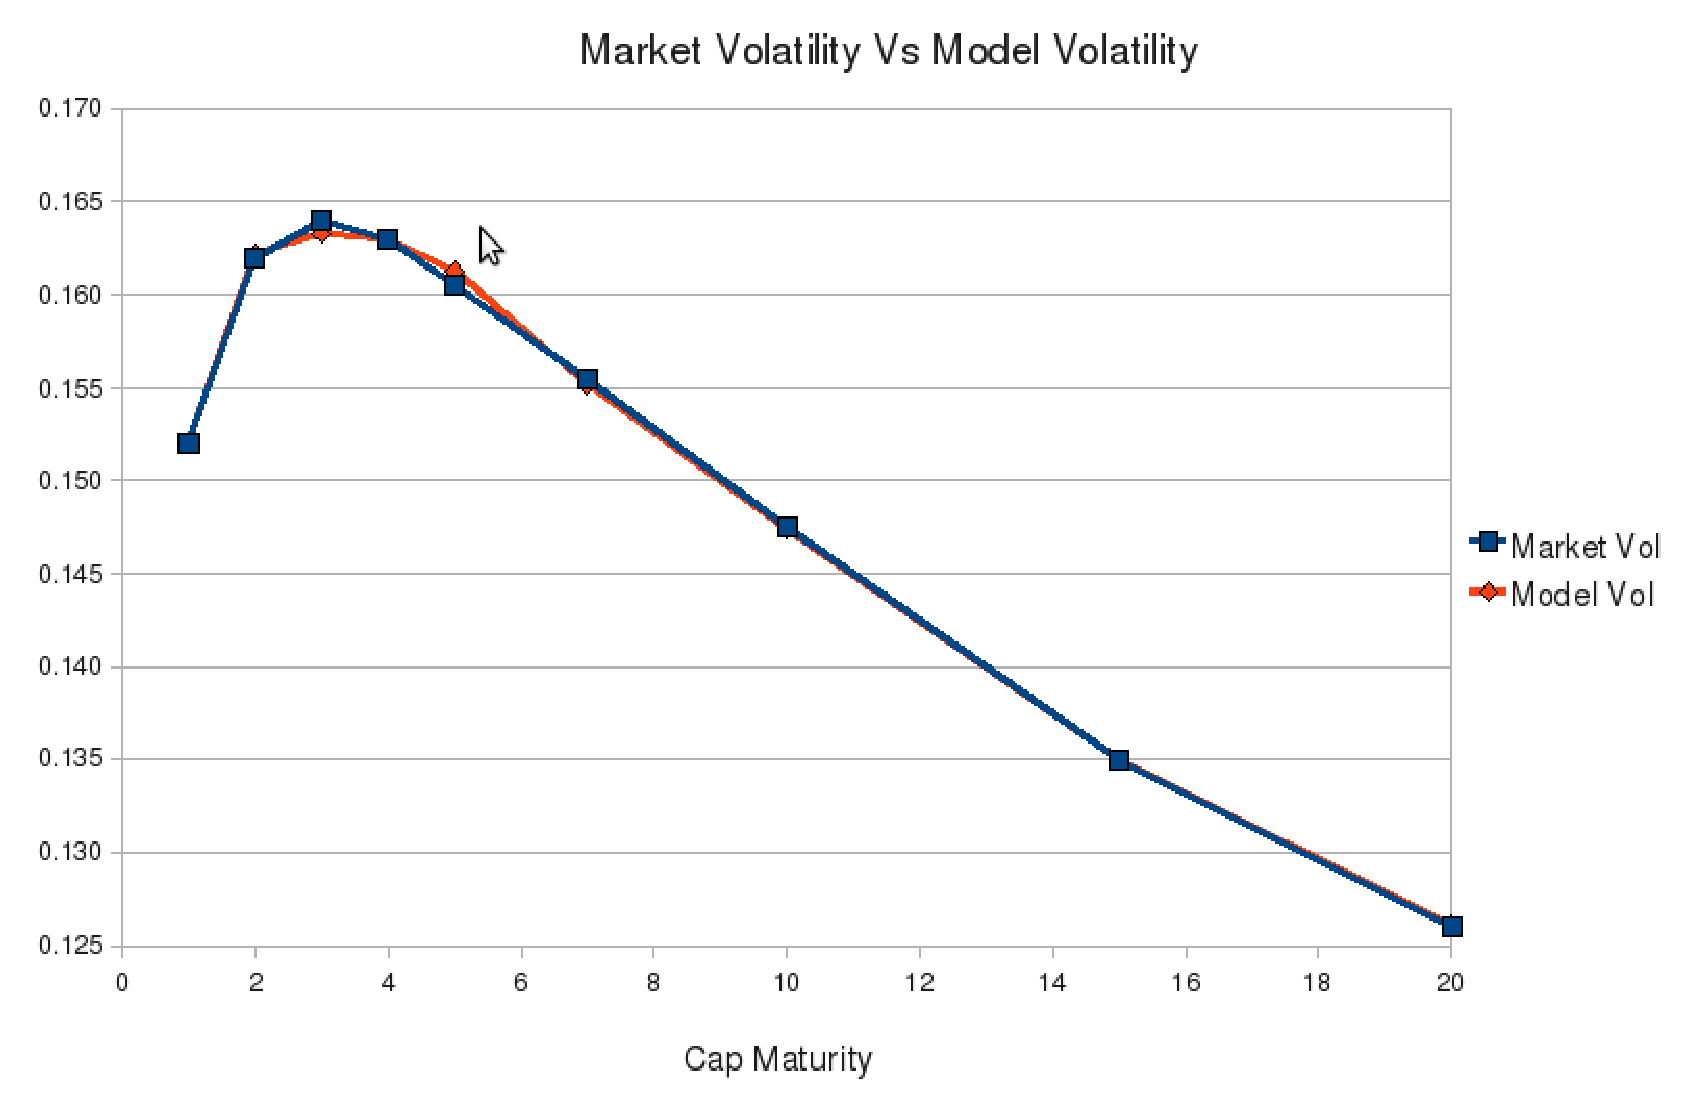
\includegraphics[width=15cm,bb=0 0 791 510,keepaspectratio=true]{cap.eps}
 % cap.eps: 791x510 pixel, 72dpi, 27.90x17.99 cm, bb=0 0 791 510
 \caption{Cap volatility curves implied by HW 2-factor model calibrated to market cap volatility curve}
 \label{fig:cap_vol}
\end{figure}

We note by \texttt{BM Volatility} the volatility found by Brigo/Mercurio in their book and by \texttt{Our Volatility} the volatility that we recover from our own calibration. The calibration execution takes a fews seconds.

As noted in \cite{BM}, the correlation parameter $\rho$ is close to 1 so that the model tends to degenerate into a one factor (non-Markov) short rate model. This can be explained by the fact that cap prices do not depend on the correlation between forward rates, knowing that a two factor model, contrary to a one- factor model, introduces correlation between forward rates.

\subsection{Second example : calibration to swaption volatility}
In this example, we consider the swaption-volatility matrix shown in table \ref{''swaption data''} below. Swaption maturities are one, two, three, four, five, seven and ten years, and the tenors of the underlying swaps go from one to ten years.

\begin{table}[''h'']
   \centering
    \begin{tabular}{|c|c|c|c|c|c|c|c|c|c|c|}
    \hline
    & 1y & 2y & 3y & 4y & 5y & 6y & 7y & 8y & 9y & 10y\\
    \hline
    1y & 0.1640 & 0.1550 & 0.1430 & 0.1310 & 0.1240 & 0.1190 & 0.1160 & 0.1120 & 0.1100 & 0.1070 \\
    2y & 0.1600 & 0.1500 & 0.1390 & 0.1290 & 0.1220 & 0.1190 & 0.1160 & 0.1130 & 0.1100 & 0.1080 \\
    3y & 0.1570 & 0.1450 & 0.1340 & 0.1240 & 0.1190 & 0.1150 & 0.1130 & 0.1100 & 0.1080 & 0.1060 \\
    4y & 0.1480 & 0.1360 & 0.1260 & 0.1190 & 0.1140 & 0.1120 & 0.1090 & 0.1070 & 0.1050 & 0.1030 \\
    5y & 0.1400 & 0.1280 & 0.1210 & 0.1140 & 0.1100 & 0.1070 & 0.1050 & 0.1030 & 0.1020 & 0.1000 \\
    7y & 0.1300 & 0.1190 & 0.1130 & 0.1050 & 0.1010 & 0.0990 & 0.0970 & 0.0960 & 0.0950 & 0.0930 \\
    10y & 0.1160 & 0.1070 & 0.1000 & 0.0930 & 0.0900 & 0.0890 & 0.0870 & 0.0860 & 0.0850 & 0.0840 \\
    \hline
\end{tabular}
\caption{\label{''swaption data''} At-the-money Euro swaptions-volatility quotes on 12/02/2001. }
\end{table}

We minimize the sum of the squares of the percentage differences between model and market swaption prices and get the following parameters :
$$a = 0.811494,\; \sigma_1 = 0.016763,\; b = 0.081977,\;  \sigma_2 = 0.007414,\; \rho = -0.325023 $$
, which are equivalent to the following G2++ parameters, using Brigo/Mercurio notations :
$$a = 0.811494,\; \sigma = 0.022249,\; b = 0.081977,\;  \eta = 0.010163,\; \rho = -0.701658 $$

The value of the correlation parameter $\rho$ is now far from trivial values, -1 and +1, because the swaption price depend on the correlation between forward rates.\\

We report the calibration results in the table \ref{''swaption res 1''} that shows the fitted swaption volatilities as implied by Hull/White 2-factor model.
\begin{table}[''h'']
   \centering
    \begin{tabular}{|c|c|c|c|c|c|c|c|c|c|c|}
    \hline
       & 1y & 2y & 3y & 4y & 5y & 6y & 7y & 8y & 9y & 10y\\
    \hline
1y & 0.1848 & 0.1514 & 0.1387 & 0.1323 & 0.1273 & 0.1230 & 0.1190 & 0.1155 & 0.1122 & 0.1085 \\
2y & 0.1596 & 0.1422 & 0.1348 & 0.1295 & 0.1252 & 0.1211 & 0.1176 & 0.1142 & 0.1104 & 0.1070 \\
3y & 0.1500 & 0.1373 & 0.1305 & 0.1258 & 0.1217 & 0.1182 & 0.1149 & 0.1110 & 0.1074 & 0.1041 \\
4y & 0.1419 & 0.1307 & 0.1252 & 0.1210 & 0.1177 & 0.1145 & 0.1106 & 0.1071 & 0.1037 & 0.1006 \\
5y & 0.1327 & 0.1245 & 0.1198 & 0.1167 & 0.1137 & 0.1098 & 0.1063 & 0.1029 & 0.0999 & 0.0966 \\
7y & 0.1215 & 0.1162 & 0.1128 & 0.1087 & 0.1052 & 0.1018 & 0.0987 & 0.0952 & 0.0924 & 0.0899 \\
10y & 0.1076 & 0.1027 & 0.0992 & 0.0965 & 0.0930 & 0.0903 & 0.0879 & 0.0853 & 0.0828 & 0.0805 \\
    \hline
\end{tabular}
\caption{\label{''swaption res 1''} Hull/White 2-factor calibrated swaptions volatilities. }
\end{table}

\begin{figure}[h!]
 \centering
 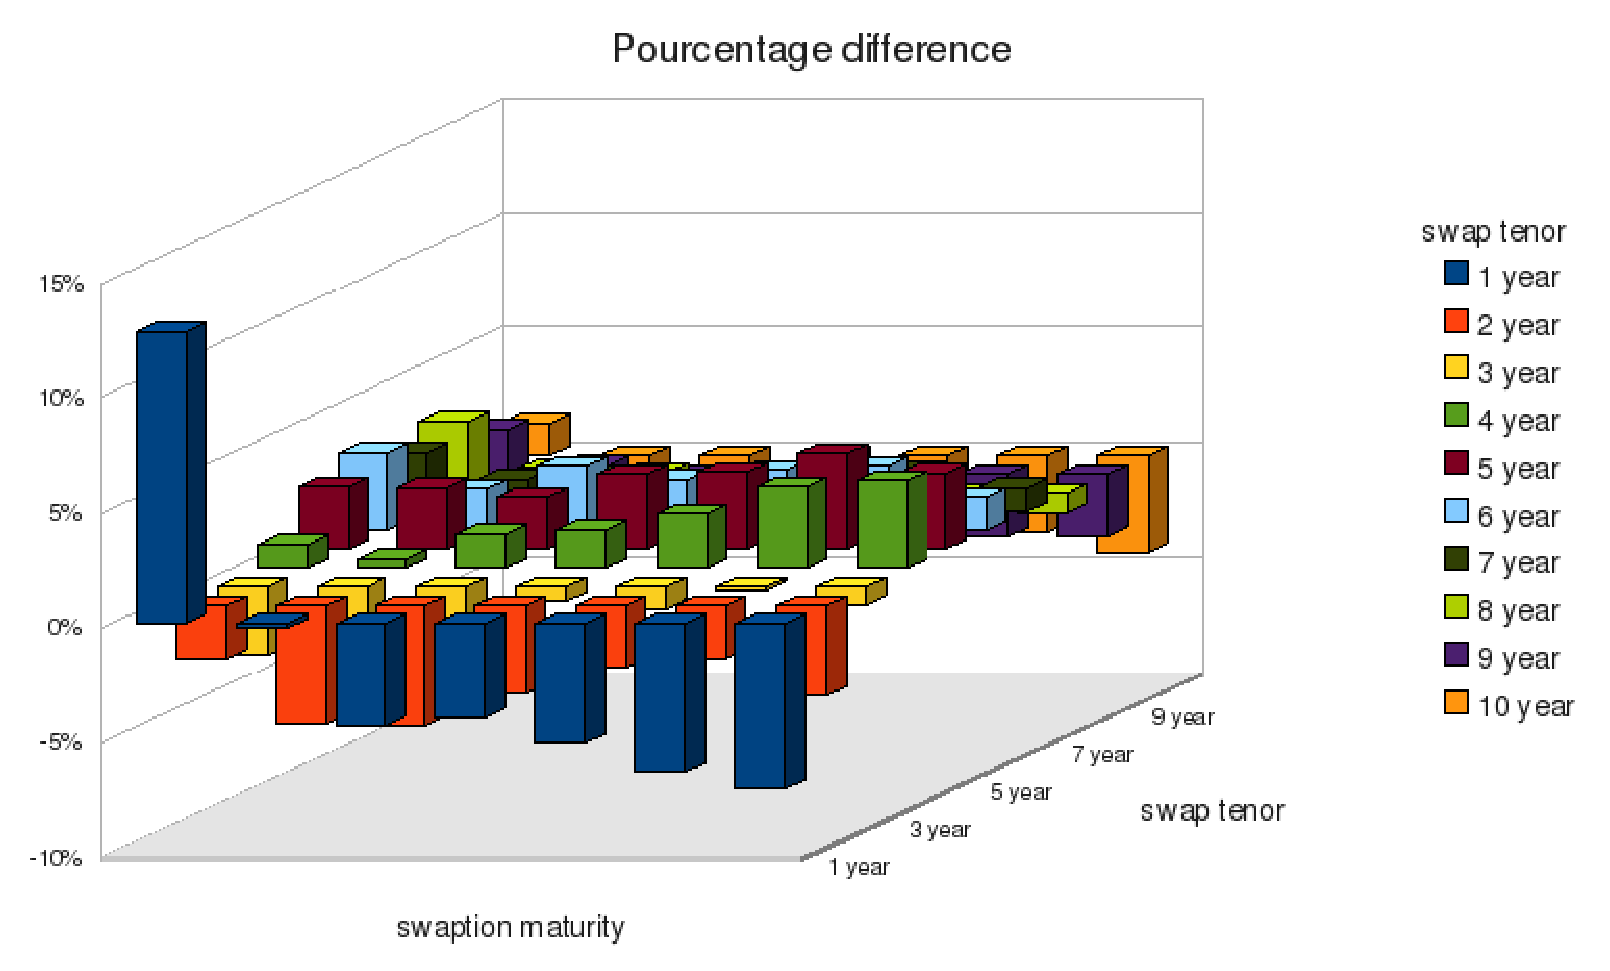
\includegraphics[width=15cm,bb=0 0 791 510,keepaspectratio=true]{swaption.eps}
 % cap.eps: 791x510 pixel, 72dpi, 27.90x17.99 cm, bb=0 0 791 510
 \caption{Swaption calibration result : Percentage difference between market and model volatilities}
 \label{fig:swaption_vol}
\end{figure}

We also plot, in the figure \ref{fig:swaption_vol}, the percentage difference between market and model volatilities :
$$
\dfrac{\text{HW2d implied volatility} - \text{market volatility}}{\text{market volatility}}
$$
This graphic shows that, except for short tenor swaption the calibration is rather satisfactory if we keep in mind that we use only five parameters to fit seventy prices

An alternative could be to only fit the most important swaptions in the matrix, specially when we need to price a product that depend on a certain set of swap rates. This will also reduce considerably the computing time, estimated by about 10mn when using the whole swaption matrix.


\newpage
\section{Conclusion}

We have presented in this project the model Hull/White two factor model and studied a practical case of calibration to market data. We have calibrated the HW 2-factor model to two sets of market data of ATM Caps volatilities and ATM Swaption volatility surfaces. The obtained results show that the model fit well the cap data and gives rather satisfactory precision when calibrating swaptions.

Another  advantage of the model is that we can construct trinomial tree for the short rate process and use it to price complex product like bermudan swaptions after calibrating the model to suitable set of swaption volatilities.


\newpage
\begin{thebibliography}{1}
\bibitem[1]{HW1d} J.Hull, A.White, \textsl{Numerical procedures for implementing term structure models I, Journal of Derivatives, Fall 1994}

\bibitem[2]{HW2d} J.Hull, A.White, \textsl{Numerical procedures for implementing term structure models II, Journal of Derivatives, Winter 1994}

\bibitem[3]{BM}  D. Brigo, F. Mercurio , \textsl{Interest Rate Models - Theory and Practice: With Smile, Inflation and Credit (Springer Finance)}

\bibitem[4]{BFGS}  Paul Armand,  J.Charles Gilbert, Sophie Jan-Jégou, \textsl{A feasible BFGS interior point algorithm for solving strongly convex minimization problems (SIAM Journal on Optimization, 11, 2000)}

\end{thebibliography}

\end{document}
